\chapter{基于工具图谱与深度优先遍历的API编排与调用方法}

\section{引言}
\label{sec:intro}

\indent 在第三章中,我们介绍了基于工具调用路径构建的API知识图谱,包括有对调用路径数据的清洗、图谱的静动态构建算法、API节点召回模型训练等部分。
尽管工具图谱能够表示大量的工具调用路径,但是仅依赖图上搜到的路径不具有灵活性,对于不同的用户需求,图上的路径不一定能够灵活满足。
同时,工具也具有生命周期和动态性,会有新建的工具或者废弃的工具,图谱上的节点也会随之变化,因此需要一种动态的API选择方法。
大语言模型能弥补这一种灵活性、动态性的缺乏,但仅依赖大语言模型的选择而不利用图谱信息,则难以解析工具之间的复杂依赖关系。

因此,我们提出了一个在工具图谱上动态遍历的算法,通过大语言模型智能体在图上动态选择节点。本章集中介绍图谱遍历和API路径选择的部分,即如何根据用户需求在大型工具图谱上进行高效的搜索和选择。
在本章主要有以下几个重要问题需要研究:
1.如何合理利用工具图谱上的依赖信息进行工具选择?
2.如何对路径选择流程进行优化,以提升整体的准确率和效率?
3.如何处理工具调用中遇到的工具调用异常、工具响应过长等问题?

\indent 针对上述问题,我们提出了一种基于工具图谱的动态寻路算法。该算法首先将用户的需求进行分析和拆解,以得到
更小的任务编排与执行单位。其次,本章提出了一种基于深度优先搜索的搜索算法,
能够实时地在图上进行搜索并选择合适的API调用路径。最后,由于API工具调用的返回结果内容较多,本着减少大语言模型推理时间与提升系统效率的考虑,
我们提出了一种响应内容压缩方法,通过让模型选择重要的字段来生成更短的响应结果,能够有效保留重要信息并提升交互效率。

\section{整体框架}

图~\ref{fig:ch4-framework}展示了本章提出的基于深度优先遍历算法的动态工具编排算法的整体技术框架。

\begin{figure}[!htp]
  \vspace{1em}
  \centering
  \setlength{\abovecaptionskip}{10pt} % 控制图片和caption之间的距离
  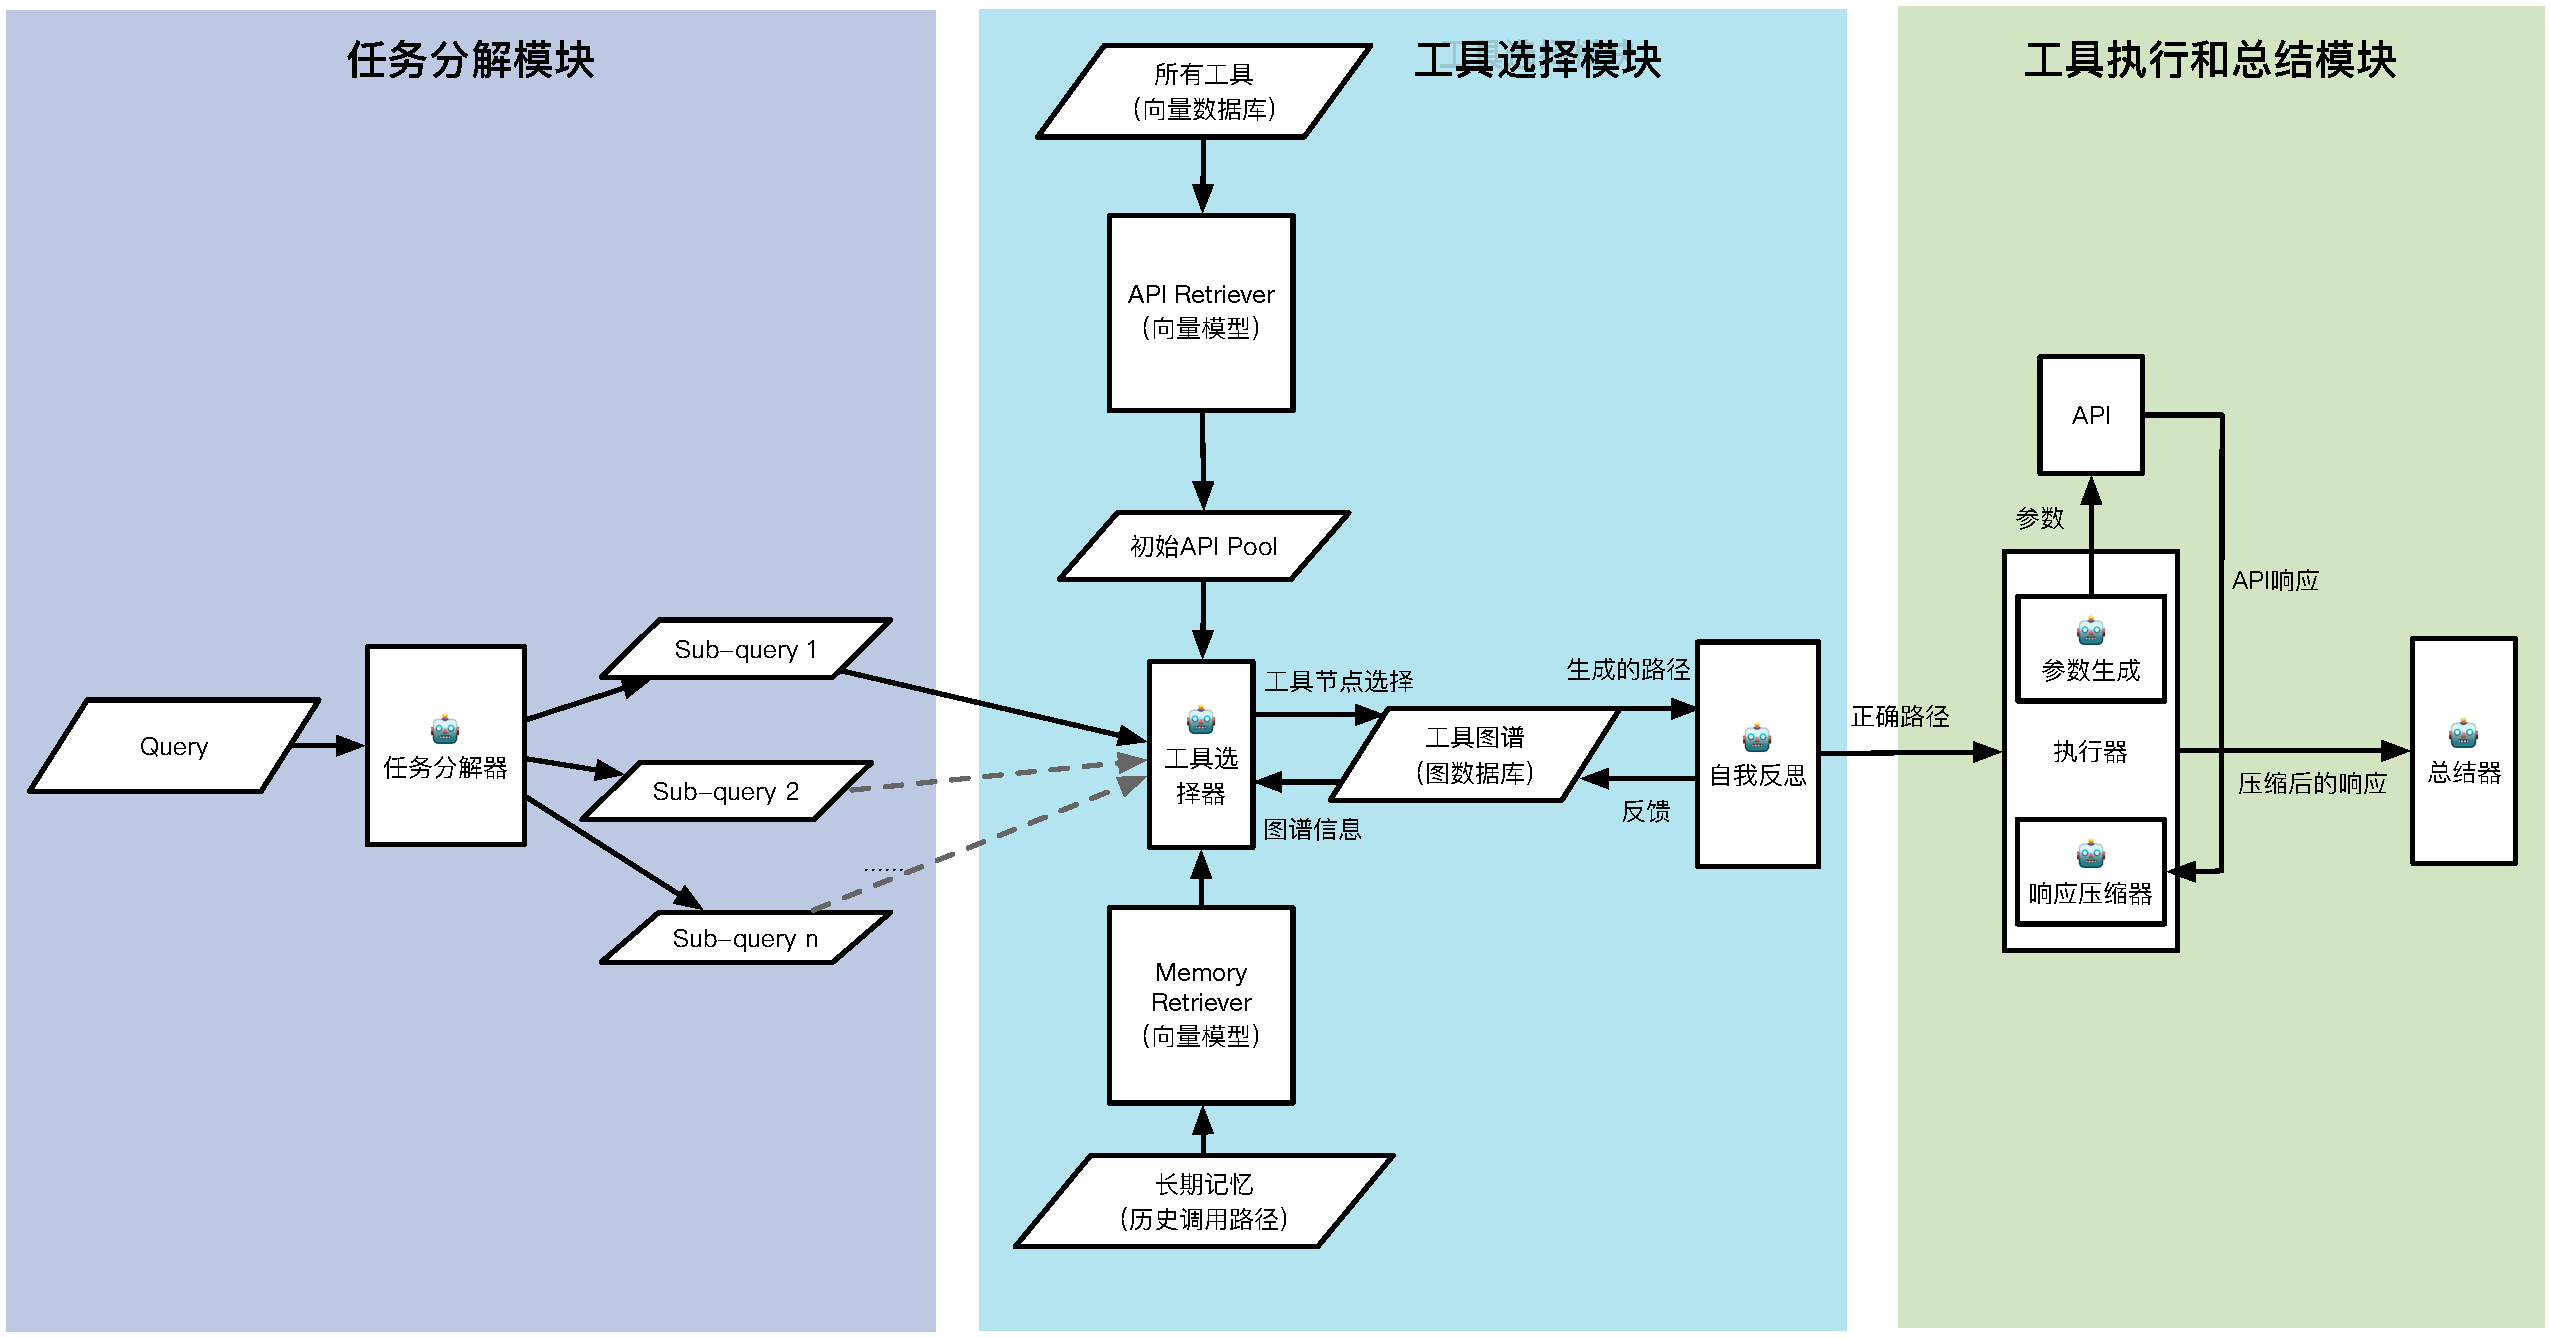
\includegraphics[height=7cm]{../assets/ch4-整体框架图-3.pdf}
  \bicaption{整体框架}{Overview of the Dynamic Tool Selection Framework}
  \label{fig:ch4-framework}
\end{figure}

该方法整体由以下几个部分组成:

\begin{enumerate}
  \item \textbf{任务解耦模块}:任务解耦模块负责将复杂、模糊的用户需求解耦为多个涉及不同大类API的子任务,能够充分提高系统处理复杂任务的能力。
  \item \textbf{任务编排模块}:该部分包括基于深度优先遍历的动态工具搜索算法、自我反思机制和长短期记忆模块。
  本质上来说,该算法就是在图上进行深度优先遍历,我们将图上的节点的权值、节点的邻居点的边权等信息,以及节点工具的描述信息等全部提供给大语言模型,让模型在图上动态选择节点。
  在工具路径选择的过程中,若遇到了路径信息,我们将会进调用“自我反思机制”,即对路径上遇到的错误进行分析并基于此错误分析内容重新
  进行路径选择。模型可以选择回溯到某个中间过程,或者是从头开始寻路。
  在大语言模型智能体不断寻路的过程中,我们会维护一个“短期记忆”,即对整体寻路流程的记录。
  为了利用历史经验知识,我们添加了“长期记忆模块”,即我们会搜索类似任务的历史工具调用路径放在提示词辅助大语言模型的规划。
  自我反思机制能够通过格式化的反思提升系统的准确性,。
  \item \textbf{任务执行模块}:在得到了整体的路径后,任务执行模块负责调用工具API,并将结果进行汇总,最终输出结果。
  其中涉及到了API参数配置、API响应压缩模块。API参数配置模块直接将API工具的说明信息和所需参数信息提供给模型,让模型提供合适参数并进行校验。
  API响应压缩模块则负责对API的响应结果进行压缩,以减少响应时间,提升交互效率。
  \item \textbf{任务总结模块}:任务总结模块即对子任务的工具调用链执行结果进行汇总,输出最终结果。
\end{enumerate}

在流程上,对于每个用户需求,只会执行一次子任务解耦。但是对于每个子任务,都会执行一次动态工具搜索算法,并且会根据搜索到的工具路径执行若干次API工具,因此会多次调用API执行模块。
最后,我们通过任务总结模块对所有子任务的结果进行汇总,得到最终输出。

\section{具体实现}

\subsection{任务解耦模块}

由于用户的需求可能会较为模糊、笼统,或者在同一个需求语句中存在多个潜在的子任务。通过对用户提供的复杂需求进行解耦、改写,并生成适合执行的具体指令,这一过程使得任务变得更加明确和易于解决。

任务解耦模块的输入包括具体用户需求、子任务格式的指令、输出格式案例以及当前工具的具体分类,输出则是JSON格式的一组子任务。每个子任务都是一个独立的任务单元,包括“子任务名称”、“子任务描述”、“子任务类别”等重要信息。每个子任务都可以看作一个完整的任务进行执行。

首先,任务解耦模块的核心功能是将用户提出的复杂或模糊需求拆解为可执行的子任务。许多用户在表达需求时,往往由于信息不明确或需求过于笼统,导致系统难以直接响应。例如,用户可能提出多个相关或不相关的要求,或者在一个指令中混合了不同领域的子任务。在这种情况下,大语言模型通过对用户输入的语义分析,将任务按照逻辑和类别进行解耦。每一个子任务将独立处理,从而避免因任务过于复杂而导致系统误解或错误执行。

总的来说,基于大语言模型的任务解耦模块通过解耦复杂任务、改写用户需求,并动态调整任务规划,使得该系统在执行复杂任务时更加灵活、精准且高效。

% 设置颜色
% \definecolor{bgcolor}{RGB}{240,240,240} % 背景颜色
% \definecolor{titlecolor}{RGB}{20,20,20} % 标题背景颜色

% \begin{center}
% % 使用 tcolorbox 创建背景
% \begin{tcolorbox}[colback=bgcolor, colframe=black, width=0.8\textwidth, boxrule=0.5mm, 
% coltitle=white, colbacktitle=titlecolor, title=An Example for Response Generation with GPT-4]

% % 使文字居中

% \textbf{Instruction Prompt:} You are currently in the response generation stage. You are given the output of selected tools that can be potentially used to solve the sub-task. Your goal is to generate a response to the user question based on the results from tools and your internal knowledge.

% \textbf{User Question:} I would like to know the value of 5 ounces of gold plus 1 million AMZN stocks in CNY.

% \textbf{Return from Tool Calling:} The stock price of AMZN is 130 USD, XAU USD is 1919.7605807522993, and the exchange rate between USD and YNC is 7.24.

% \textbf{Output:} \textcolor{red}{Total value in CNY: Total value = Value of gold in CNY + Value of stocks in CNY = 69,495.87 + 941,200,000 = 941,269,495.87 CNY. Therefore, the combined value of 5 ounces of gold and 1 million Amazon stocks in Chinese Yuan is approximately 941,269,495.87 CNY.}

% \end{tcolorbox}

% \end{center}


\subsection{任务编排模块}

为了更好地利用我们构建的工具图谱,并挖掘隐藏节点关系中的知识,
我们开发了一个基于深度优先遍历的寻路算法。
与“思维链”(Chain-of-Thought)或ReACT方法相比,
该算法的优点在于该方法在图谱上进行可回溯的动态选路,能够防止错误传播的问题,
并能够对整个工具空间进行更全面的探索。
在动态选择API工具路径的同时,我们会维护一个“短期记忆”,即
当前的路径和每一步路径选择(前进/回溯)的理由。同时,为了利用历史经验知识,
我们将历史上类似的任务的正确工具路径作为提示词提供给模型,以辅助模型进行路径选择。
最后,在该算法能够通过“自我反思机制”来对路径进行判断和错误诊断,
这一机制进一步提升了路径选择的准确率。

\subsubsection{基于深度优先遍历的动态搜索算法}

图~\ref{fig:ch4-dfs}为本文提出的基于深度优先的寻路算法。

\begin{figure}[!htp]
  \vspace{1em}
  \centering
  \setlength{\abovecaptionskip}{10pt} % 控制图片和caption之间的距离
  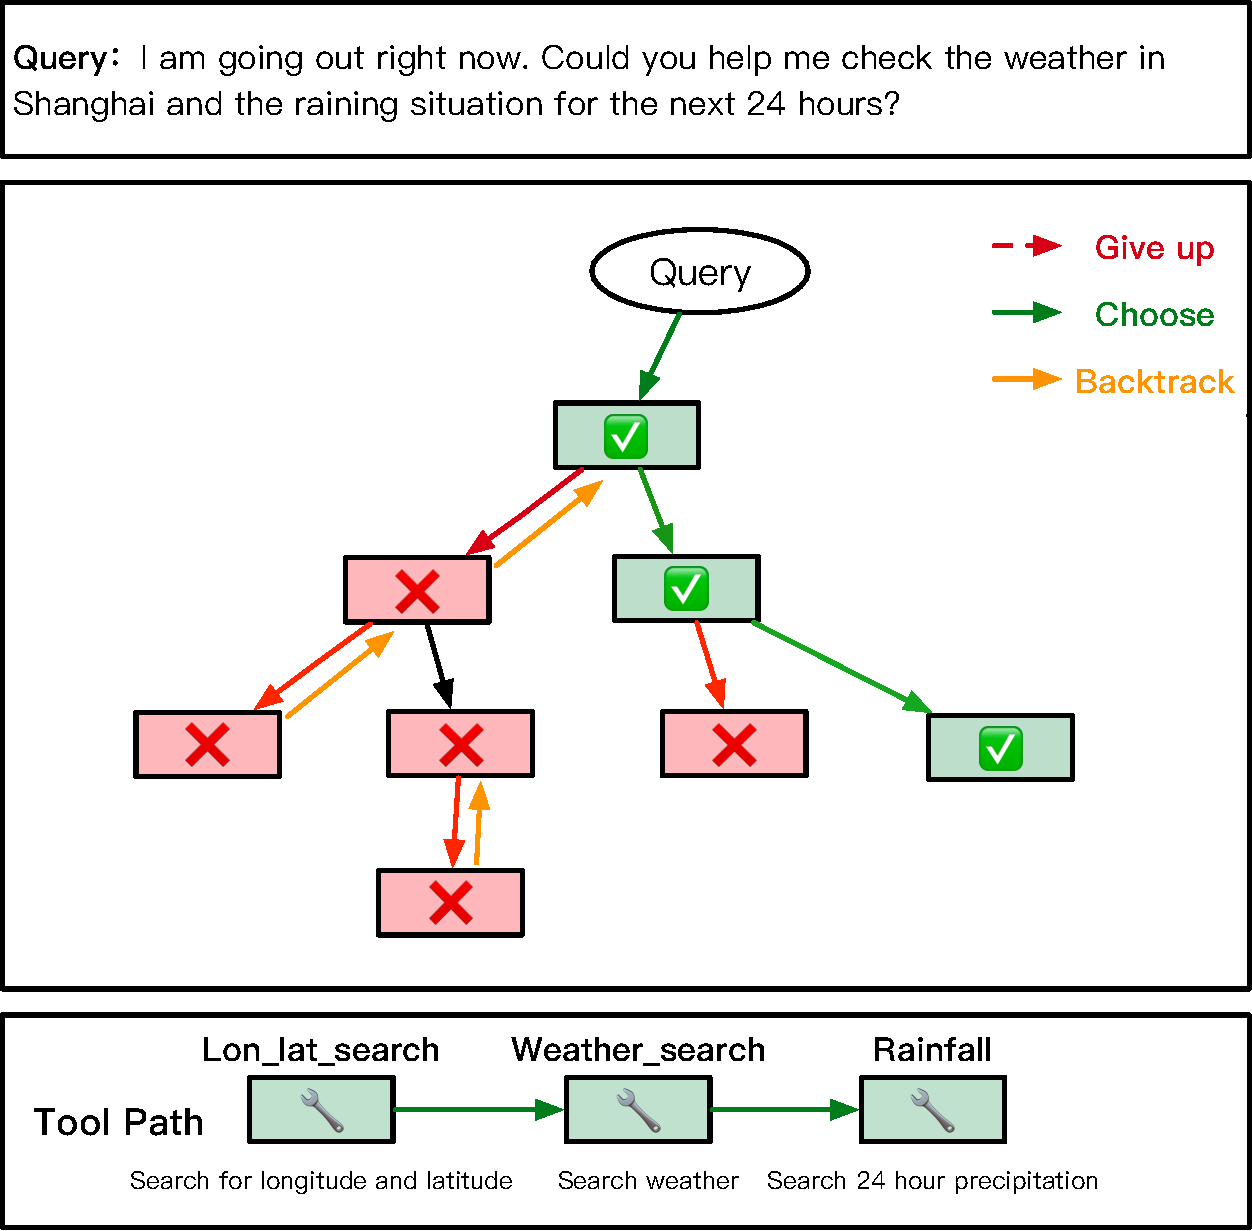
\includegraphics[height=8cm]{../assets/ch4-dfs算法.pdf}
  \bicaption{基于深度优先的寻路算法}{Dynamic DFS Search on Tool Graph}
  \label{fig:ch4-dfs}
\end{figure}

首先,由于图谱上的节点数量众多,选择初始节点是算法中非常关键的一步。
在选择初始节点时,我们训练了一个基于语义相似度的API召回器,能够根据用户的需求语句得到一组
在语义上最相似的工具作为初始工具的候选集。然后我们从中选择一个节点并开始在图上进行深度优先搜索遍历,
让模型在图上不断遍历其他节点。

具体算法逻辑如下:对于每个选择的节点,
我们将获取当前节点的邻居节点及其权值,并提供给大模型智能体,
要求大语言模型选择下一个工具节点或回溯。
对于邻居节点候选集的筛选,
我们会首先获取到图中所有邻居节点,然后
我们根据当前节点与该邻居节点的
工具转移边权进行排序,
选择边权最大的K个节点
作为候选邻居节点。
同时,我们会获取每个邻居节点的点权,
同样作为额外信息提供给大语言模型,
作为工具可用性的参考。
如果邻居节点不足K个,
我们将再次调用API召回器,以补全K个候选节点的选项。

该算法会根据当前状态继续迭代选择下一个工具节点或发起回溯,
直到模型决定结束选择或放弃该任务。

不管模型选择下一节点还是选择回溯,我们都将把模型的理由和具体操作加入短期记忆中,
将回溯步骤添加到短期记忆的原因是让模型记住在本次推理中之前采取的错误操作,
避免后续重复选择不可行的工具。
如果模型回溯到了初始节点,并且需要继续回溯,
我们可以理解为基于当前的工具选择,
该任务不可行,即放弃任务执行。

\subsubsection{初始节点召回器}

在上述算法中,除初始节点外的其他点都是根据当前节点的邻居节点及其权值来选择的。
因此,初始节点的选择是选择正确路径的关键。

由于工具图中包含大量的工具,无法让大语言模型浏览所有工具信息并选择最合适的。
因此在这里我们设计了基于语义相似度的API召回器,能够根据用户的需求语句召回一组在语义上最相似的工具作为初始工具的候选集。

通常API召回是通过向量模型和相似度算法来进行的,具体而言,我们将用户需求(查询)和每个API的信息都转化为向量表示,并通过计算查询向量与API向量之间的相似度来检索相关API。这个过程首先使用预训练的语言模型将API的文本描述转化为向量,这些向量能够捕捉文本的语义信息。接着,通过计算查询向量与API向量之间的相似度,常用的相似度度量包括余弦相似度和欧氏距离,系统会召回与查询最相关的若干个API,通常会设置一个阈值,以确保返回的结果在一定的相似度范围内。随后,对召回的API进行排序,通常按照相似度从高到低排列,以便优先展示最相关的结果。在某些情况下,可以结合额外的规则或业务逻辑进一步优化结果,例如排除某些不相关的API或添加领域特定的过滤条件。

然而,我们在实际应用中发现,针对一些模糊的用户需求,开源的向量模型在召回工具列表时往往会收到噪声的影响。

如图~\ref{fig:why-tune}所示,在工具召回时,有很多噪声工具被召回,而真正对任务有用的工具排名靠后。

\begin{figure}[!htp]
  \vspace{1em}
  \centering
  \setlength{\abovecaptionskip}{10pt} % 控制图片和caption之间的距离
  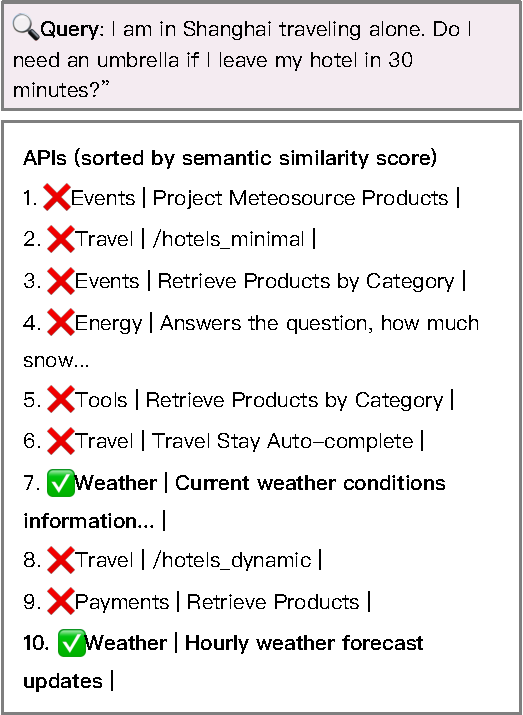
\includegraphics[height=8cm]{../assets/ch3-为何需要微调.pdf}
  \bicaption{使用开源向量模型得到的API排序结果}{API Ranking Using Open-source Embedding Models}
  \label{fig:why-tune}
\end{figure}

因此,为了解决上述问题,本文提出了基于通用向量模型进行微调,通过构造高质量的工具训练数据来将领域知识注入模型,从而提升模型在工具选择上的准确性。

在训练向量模型时,训练数据包含三个部分:正样本,负样本,查询语句。
查询语句即为数据集中的“query”字段,对应用户输入的查询信息。
正样本也可以直接使用数据集提供的参考API列表。

对于负样本的部分,如图~\ref{fig:negative-sample-generation},我们采取了两种不同的负样本构造方式:
一种是简单负样本(Simple Negative)构造,另一种是困难负样本构造(Hard Negative)。

\begin{figure}[!htp]
  \vspace{1em}
  \centering
  \setlength{\abovecaptionskip}{10pt} % 控制图片和caption之间的距离
  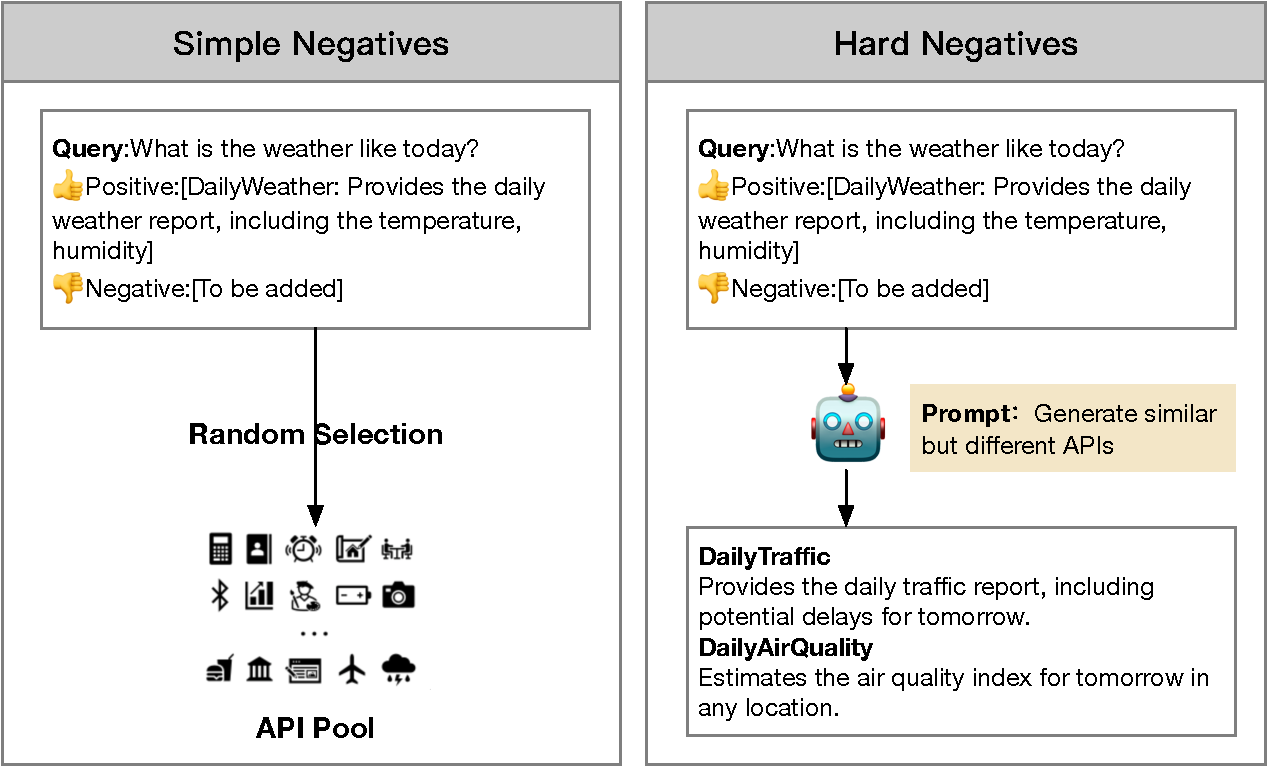
\includegraphics[height=7cm]{../assets/ch3-负样本构造.pdf}
  \bicaption{负样本构造的两种方式}{Negative Sample Generation}
  \label{fig:negative-sample-generation}
\end{figure}

\indent \textbf{简单负样本构造}。对于简单负样本构造,我们直接选择不同类别的K个工具作为负样本。
在简单负样本构造中,不同类别的API之间的功能上一般有区别,因此简单负样本构造能够保证负样本与正样本之间在工具上的差异。

\indent \textbf{困难负样本构造}。在工具选择、调用场景,开源的通用向量模型难以区分工具之间细微的语义区别。
困难负样本构造的目的是帮助模型更好地区分工具之间细微的语义区别,帮助更好地应对噪声。
我们选择采用GPT-3.5完成困难负样本的构造。由于原工具数据量众多,
从中筛选语义表述类似、但是功能上有区别的工具样本费时费力。
因此我们采取了直接用大语言模型生成工具描述作为负样本的策略。

具体策略如下:
首先,我们采样一批<query,推荐工具集>的数据,
然后我们遍历其中的推荐工具集的工具,
通过提示词将用户需求和工具描述提供给大语言模型,
要求模型生成类似但是功能上无法满足用户需求的工具描述。
通过这样遍历工具描述生成负样本,可以生成一组高质量的困难负样本供模型学习。

\subsubsection{自我反思机制}

自我反思机制的主要目的是对生成的工具调用路径进行反思,以提升整体的准确率。

自我反思机制的触发时间点有三个:1.动态寻路算法找到路径并主动结束路径 2.动态寻路算法超过了最大迭代次数并终止或放弃寻路

具体而言,自我反思模块的输入是
我们当前的工具调用路径和用户需求,
根据API工具召回器召回的初始节点,
以及我们撰写的反思格式说明。
输出包括以下几部分:1.成功/部分失败/完全失败的等级 2.若部分失败,从哪一个工具节点开始为首个错误节点 3.若全部失败,有哪些可以删除的噪声工具初始节点

评价为“成功”的路径,我们直接进入API调用模块进行调用。
对于评价为“失败”的路径,我们
会根据失败的等级选择进行不同的重新寻找工具调用路径:
第一种是从中间步骤开始重新寻找路径,
另一种是从头开始重新寻找路径。

\begin{enumerate}
  \item \textbf{从中间步骤继续}: 在任务未完成的情况下,我们将在短期记忆中记录寻路过程中的每一步的选择节点和理由。
  当路径被标记为“放弃”或被评判器认定为“失败”时,我们会重新激活该路径上的智能体,
  并将识别到的失败原因重新纳入历史上下文。
  评判器在判定“失败”时,通常会标记出它认为的第一个出现错误的节点。
  在重新激活智能体并进行寻路时,我们将从该节点继续,
  而不是从头开始。这种从中间步骤继续的策略不仅能够加快寻路速度,
  减少大语言模型的调用次数,还能充分利用先前成功调用的经验,
  从而提升决策的准确性。
  \item \textbf{重新寻路}: 在自我反思模块认为路径“完全失败”时,
  我们需要从头开始重新生成整条路径。评判器会识别路径初始节点中与用户查询无关的工具名称作为反思的一部分。
  为了提高系统的整体效率,我们会首先从初始工具节点中移除这些无关的工具,
  避免大模型受到这些噪声的影响,从而选择无关的工具进行调用,
  导致后续调用出错。通过这一清理过程,我们能够有效减少噪声工具的影响,
  确保后续搜索的准确性。\par
  接下来,我们将会在经过噪声清理的工具组中重新开始选择下一节点并组成路径。
  这种从头开始的自我反思允许算法在一个更加简洁与优化的初始条件下进行搜索,
  从而提升工具调用路径的质量与响应速度。
\end{enumerate}
 
该自我反思机制可以反复应用,直至满足终止条件为止。这种持续的反思过程确保了对问题的逐步优化,有助于形成更加有效的调用路径。

综上所述,这两种反思策略——从中间步骤继续优化和从头开始的寻路——的结合使用,能够在处理用户需求未满足的情况下,提供更高的灵活性与效率。
通过不断的反思与优化,系统将逐步提升其在动态环境中的适应能力,确保用户体验的持续改进。

\subsubsection{工具调用路径长短期记忆框架}

本小节提出了关于增强模型规划和推理准确性的长短期记忆框架。该框架主要分为短期记忆和长期记忆两个部分。
短期记忆部分指的是当模型在图上动态推理时存储的每个步骤的记录,
主要聚焦于以什么数据格式来存储推理步骤,
以及记录哪些有用的记忆信息:在图上前进、回溯还有大模型的思考过程等。
长期记忆部分主要是将历史的工具调用路径存储在数据库中,通过相似度搜索算法加入到工具选择器
的提示词中,以增强其推理和规划能力。

\indent \textbf{短期记忆}

短期记忆指的是模型在图上进行不断推理时保存的一些状态信息,
这些信息包括:用户的任务、当前遍历到的节点、历史遍历的节点、调用路径信息等。
在遍历的过程中,我们会动态地更新和维护短期记忆存储的内容,来辅助模型进行推理和规划。
在短期记忆中,我们一般将全部的信息存储在内存中,
然后每次直接构建提示词添加到大语言模型的上下文中,
让模型能够感知到当前的状态和环境。

\indent \textbf{长期记忆}

长期记忆与短期记忆相对,是固定存储在数据库中的信息,且会随着调用次数的增加不断积累。
它记录最终形成的工具调用链和结果,每次推理时,系统都会从长期记忆库中搜索,将搜到的相似需求的工具调用路径提供给
工具选择器,利用历史经验辅助大语言模型的推理。

长期记忆模块基于检索增强生成(Retrieval-Augmented Generation, RAG)逻辑,通过将历史上成功的<用户需求,工具调用路径>转为向量存储。新需求通过向量模型转为嵌入向量,并与数据库中的向量进行相似度计算。系统会根据相似度排序,检索出与当前需求最相似的 K 个历史需求及其工具调用路径。最终,这些<用户需求,工具调用路径>的二元组会被加入大语言模型的上下文中,辅助推理与规划。

\subsection{工具调用模块}
\label{sec:real_tool_simulation}

\subsubsection{整体逻辑}

工具调用模块的主要功能是执行规划好的API调用路径,并将得到的结果返回给系统,
从而为后续的推理和规划提供支持,最终生成符合用户需求的答案。

该模块的整体逻辑可以分为两个主要部分:工具调用和工具响应解析。
具体而言,我们首先根据工具的描述信息和用户需求生成API调用的参数,然后通过代码生成请求体并通过API调用接口将请求体发送给目标API工具,
以获取其响应。
获得响应后,理论上我们可以直接将所有工具的调用结果直接提供给总结器,要求模型根据所有的API响应输出最终结果。

但由于每个响应的长度参差不齐,对于一些响应长度较长的API工具,可能单个API的响应数据就超出了大语言模型的上下文限制。
因此,我们添加了一个基于大语言模型的响应压缩模块,通过对响应的压缩,将API响应的字符数控制在1024个字符以内,以缓解大语言模型的上下文限制。

\subsubsection{工具参数生成}

工具调用模块的主要工作就是生成API工具的请求体。在请求体的生成过程中,我们首先将与工具调用相关的内容提供给大语言模型智能体,要求其生成指定的JSON格式调用输入,包括但不限于工具调用的URL、所需输入参数及工具的登录验证信息等。接着,我们对生成的JSON数据中的参数信息进行验证,并确定请求体中各个参数的结构和格式。

首先,我们会确认生成的参数URL与工具库中的URL是否匹配。其次,参数的正确性对API工具调用的成功至关重要,因此在执行调用工具代码之前,我们会对参数进行严格的校验。在这一步中,我们验证具体的参数数量、类型和名称,并对这些部分进行精确匹配。如果缺少必要的参数或参数类型不匹配,我们将返回固定的错误信息,并要求参数解析器重新生成参数。这一过程会一直重复,直到获取正确的参数或超过最大尝试次数后放弃该API调用。

在成功验证URL和参数后,我们将调用固定的函数来执行API请求,并获取JSON格式的响应,随后将其提供给响应解析模块。

\subsubsection{工具响应解析模块}

生成请求体后,我们将其通过API调用接口发送给目标API工具,以获取相应的响应数据。响应数据通常是以JSON格式返回的,这其中可能包含大量的信息,而这些信息并不总是直接相关。在我们的实际实验中,我们通过分析发现许多API返回内容包含大量冗余信息,导致其长度过长,无法将调用结果输入到大语言模型中,直接使用大语言模型从中提取重要信息较为困难。因此,我们对API的响应结果进行了压缩。该模块的目标是在尽可能多地保留关键信息的同时减少API响应的长度,便于放入大语言模型的上下文中。

由于每个API的响应格式不是固定的,无法确定每个字段应该舍弃还是保留,因此我们采用大语言模型来分析示例响应,仅保留与用户需求相关的字段,以减小响应长度。

如图~\ref{fig:ch4-compression},响应压缩的逻辑如下所示:

\begin{figure}[!htp]
  \vspace{1em}
  \centering
  \setlength{\abovecaptionskip}{10pt} % 控制图片和caption之间的距离
  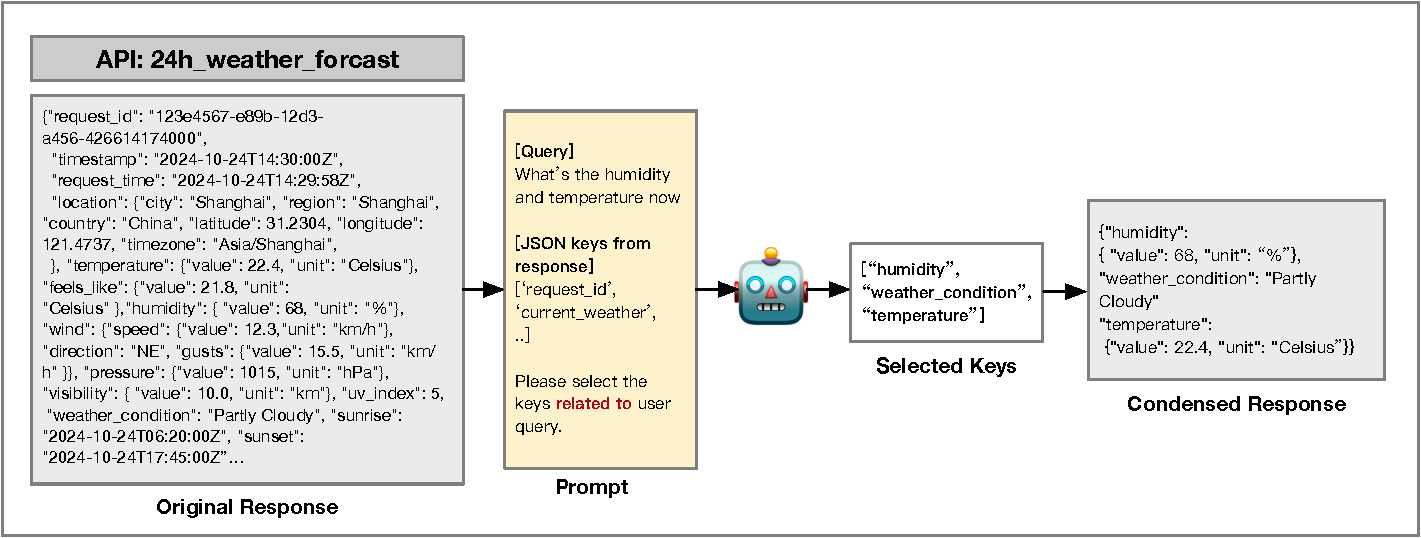
\includegraphics[height=4cm]{../assets/ch4-响应压缩.pdf}
  \bicaption{响应压缩模块}{Compression of API responses}
  \label{fig:ch4-compression}
\end{figure}

\begin{enumerate}
    \item \textbf{工具文档信息}:所有API工具均来自ToolBench等开源数据集,这些数据集同时包含每个API的详细描述信息和API响应示例。因此,我们可以将工具名称、工具描述、API名称、API描述、参数及API响应示例的内容以文本形式提供给大型语言模型。这部分构成了压缩模块的基本提示词。
    
    \item \textbf{详细规则指令}:我们要求大型语言模型仔细阅读API的功能描述,并保留与功能描述最相关的信息,诸如API版本、调用时间或无效信息等可以被舍弃。
    
    \item \textbf{上下文学习示例}:我们使用了三个上下文学习示例,每个示例由一个原始API响应和对应的专家撰写的压缩响应组成。我们要求压缩器以自然语言文本格式输出所有需要保留的字段,然后通过正则表达式匹配得到一个保留字段的列表,并用固定的代码逻辑筛选出相应字段的返回内容。
\end{enumerate}

在推理过程中,当API响应长度超过1024个字符时,我们会通过移除不重要的信息来压缩响应。如果压缩后的响应仍然超过1024个字符,则只保留压缩后的前1024个字符。这种方法能够有效地减少API响应长度,对API响应进行去噪。同时,也能够缓解大型语言模型有限的上下文窗口的问题,确保系统的正常调用。

通过分析我们在ToolBench中的API响应示例,其中一个API的平均响应字符串长度为xxx个字符。经过响应压缩后,最长的响应也不超过1024个字符。通过这种方式,我们有效降低了xx\%的超出上下文的情况,平均每个API响应结果节约了xx个字符。

\subsection{工具总结模块}

【主要就写对所有API的调用结果进行总结,重要的是如何进行错误处理和拒答】

【看看其他论文咋写的】


\section{本章小结}
\label{sec:summary_chap4}